% !TEX TS-program = xelatex
% !TEX encoding = UTF-8 Unicode
\documentclass[11pt,a4paper]{article}
\usepackage{amsmath,amssymb}
\usepackage{empheq}
\usepackage[semibold]{ebgaramond}
\usepackage[cmintegrals,cmbraces]{newtxmath}
\usepackage{ebgaramond-maths}
\usepackage{bm}
\usepackage[OMLmathrm, OMLmathsfit, rmdefault=mdugm]{isomath}
\usepackage{tocbibind}
\usepackage{graphicx}
\graphicspath{{./pics/}}
\usepackage{wrapfig}
\usepackage{capt-of}

\makeatletter
  \DeclareSymbolFont{ntxletters}{OML}{ntxmi}{m}{it}
  \SetSymbolFont{ntxletters}{bold}{OML}{ntxmi}{b}{it}
  \re@DeclareMathSymbol{\leftharpoonup}{\mathrel}{ntxletters}{"28}
  \re@DeclareMathSymbol{\leftharpoondown}{\mathrel}{ntxletters}{"29}
  \re@DeclareMathSymbol{\rightharpoonup}{\mathrel}{ntxletters}{"2A}
  \re@DeclareMathSymbol{\rightharpoondown}{\mathrel}{ntxletters}{"2B}
  \re@DeclareMathSymbol{\triangleleft}{\mathbin}{ntxletters}{"2F}
  \re@DeclareMathSymbol{\triangleright}{\mathbin}{ntxletters}{"2E}
  \re@DeclareMathSymbol{\partial}{\mathord}{ntxletters}{"40}
  \re@DeclareMathSymbol{\flat}{\mathord}{ntxletters}{"5B}
  \re@DeclareMathSymbol{\natural}{\mathord}{ntxletters}{"5C}
  \re@DeclareMathSymbol{\star}{\mathbin}{ntxletters}{"3F}
  \re@DeclareMathSymbol{\smile}{\mathrel}{ntxletters}{"5E}
  \re@DeclareMathSymbol{\frown}{\mathrel}{ntxletters}{"5F}
  \re@DeclareMathSymbol{\sharp}{\mathord}{ntxletters}{"5D}
  \re@DeclareMathAccent{\vec}{\mathord}{ntxletters}{"7E}
\makeatother

\usepackage{array}
\usepackage{enumitem}
% to produce a comma between multiple footnotes / https://tex.stackexchange.com/questions/40072/incompatibility-between-footmisc-option-multiple-and-hyperref/62091#62091
\let\oldFootnote\footnote
\newcommand\nextToken\relax
\renewcommand\footnote[1]{%
    \oldFootnote{#1}\futurelet\nextToken\isFootnote}
\newcommand\isFootnote{%
    \ifx\footnote\nextToken\textsuperscript{,}\fi}

\defaultfontfeatures{Ligatures=TeX} % makes this a feature for all selected fonts
\usepackage{esint}
\usepackage{polyglossia}
\setmainlanguage{english}
\usepackage[text={18cm,26cm},centering]{geometry} % 
\usepackage{natbib}
\usepackage{mdframed}
\usepackage{lipsum}
\usepackage[usenames,dvipsnames,svgnames,table]{xcolor}
\usepackage{hyperref}
\usepackage{url}
\usepackage{pdfpages}
\usepackage[export]{adjustbox}

\hypersetup{
  colorlinks,
  citecolor=bleuSU,
  linkcolor=bleuSU
}
\definecolor{bleuSU}{RGB}{26,39,101}

\usepackage[normalem]{ulem}
\makeatletter
\renewcommand*{\uuline}{%
  \bgroup
  \UL@setULdepth
  \markoverwith{%
    \lower\ULdepth\hbox{%
      \kern-.03em%
      \vtop{%
        \hrule width.2em%
        \kern 0.6pt % distance between the two underlines
        \hrule
      }%
      \kern-.03em%
    }%
  }%
  \ULon
}
\makeatother
\setlength{\ULdepth}{-2pt}  % distance from double underline to letter

\usepackage{environ}
\newtoggle{corrige}

\NewEnviron{answer}{%
  \iftoggle{corrige}
    {\begin{mdframed}\textbf{Answer: } \BODY\end{mdframed}}
    {}%
  }

\newcommand{\delS}{\delta S}
\newcommand{\delA}{\delta A}
\newcommand{\delh}{\delta h}
\newcommand{\delt}{\delta t}
\newcommand{\delz}{\delta z}
\newcommand{\delbx}{\delta \matrixsym x}
\newcommand{\lp}{\left(}
\newcommand{\rp}{\right)}
\newcommand{\itA}{\textit A}
\newcommand{\itB}{\textit B}
\newcommand{\dAB}{\mathcal D_{AB}}
\newcommand{\bA}{\matrixsym A}
\newcommand{\bff}{\matrixsym{f}}
\newcommand{\bF}{\matrixsym{F}}
\newcommand{\bj}{\matrixsym{j}}
\newcommand{\bJ}{\matrixsym J}
\newcommand{\bn}{\matrixsym{n}}
\newcommand{\bN}{\matrixsym N}
\newcommand{\bP}{\matrixsym{P}}
\newcommand{\br}{\matrixsym r}
\newcommand{\bt}{\matrixsym t}
\newcommand{\be}{\matrixsym e}
\newcommand{\bu}{\matrixsym u}
\newcommand{\bv}{\matrixsym v}
\newcommand{\bw}{\matrixsym w}
\newcommand{\bx}{\matrixsym x}
\newcommand{\pd}[2]{\frac{\partial #1}{\partial #2}}
\newcommand{\D}[2]{\frac{D #1}{D #2}}
\newcommand{\dd}[2]{\frac{\mathrm d #1}{\mathrm d #2}}
\newcommand{\dA}{\mathrm dA}
\newcommand{\dV}{\mathrm dV}
\newcommand{\dS}{\mathrm dS}
\newcommand{\prg}[1]{\paragraph{$\rhd$ #1}}
\newcommand{\alphaijkl}{\alpha_{ijkl}}
\newcommand{\Aijkl}{A_{ijkl}}
\newcommand{\delij}{\delta_{ij}}
\newcommand{\sigij}{\sigma_{ij}}
\newcommand{\sigji}{\sigma_{ji}}
\newcommand{\sigxy}{\sigma_{xy}}
\newcommand{\matL}{\mathcal L}
\newcommand{\matO}{\mathcal O}
\newcommand{\matS}{\mathcal S}
\newcommand{\kij}{k_{ij}}
\newcommand{\tensor}[1]{\smash{\uuline{#1}{}}}
\setlength{\parindent}{0pt} % remove indent

\setlist[enumerate]{topsep=0pt,itemsep=-1ex,partopsep=1ex,parsep=1ex}

\begin{document}
\setlength{\unitlength}{1cm}
\noindent
\parbox{\textwidth}{
\textsc{
Sorbonne Université  
\hfill
Year 2022-2023
}
}
\parbox{\textwidth}{
\textsc{
Faculté des Sciences
\hfill
Physics of Fluids \& Nonlinear Physics
}
}

\begin{center}
\Large
\textbf{Hydrodynamics} \\ 
\textsl{Tutorial 4: lava flows and viscous slumping} \\[1ex]
\end{center}

\section{The spreading of a viscous lava flow \citep{Huppert1982}}
\begin{figure}[ht]
    \centering
    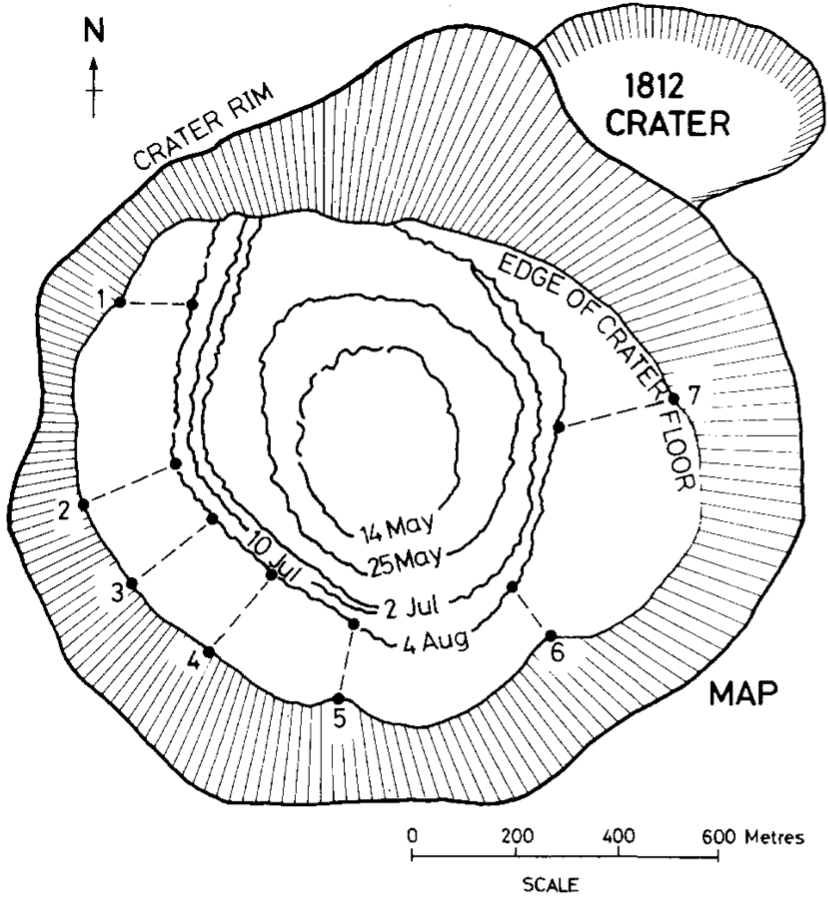
\includegraphics[width=5cm,valign=m]{soufriere.png}
    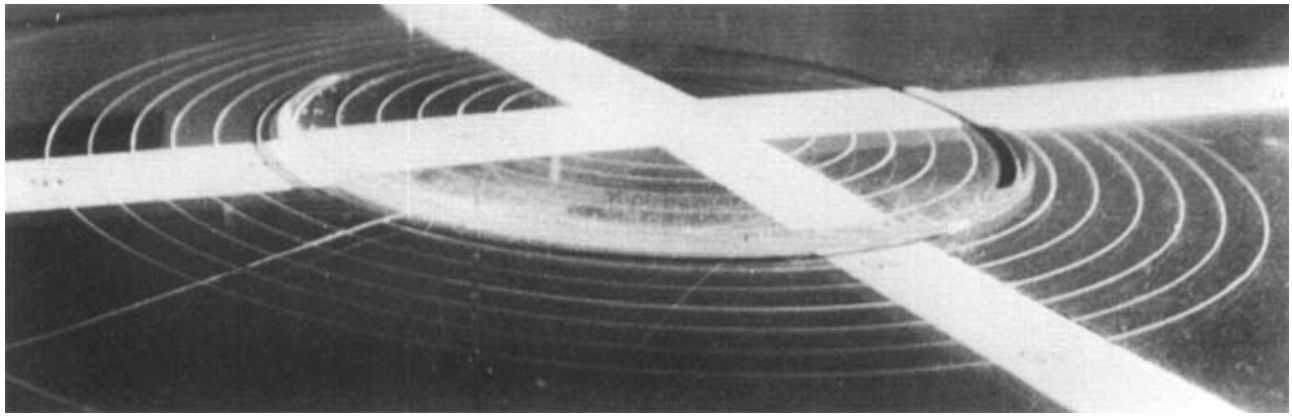
\includegraphics[width=10cm,valign=m]{silicon_oil.png}\\
    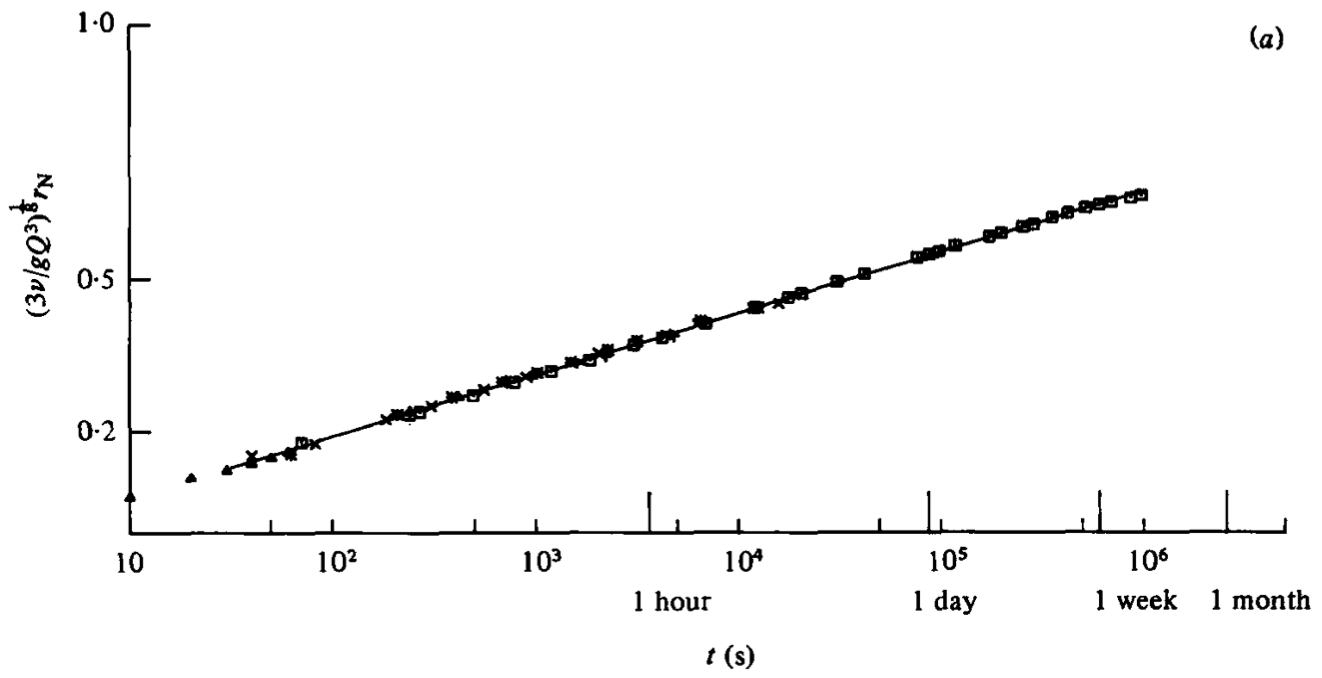
\includegraphics[width=7cm,valign=m]{spreading_law.png}
    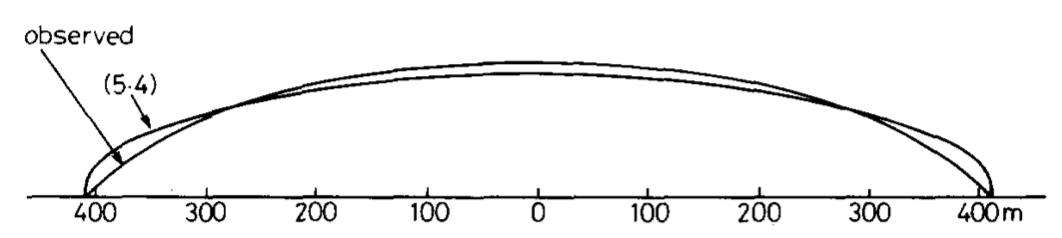
\includegraphics[width=7cm,valign=m]{lava_flow_model.png}
    \caption{\textbf{Lava flow modelling.} Top left: evolution of lava spreading during the 1979 Soufrière's eruption. Top right: spreading of a 400 cm$^3$ volume of silicone soil with $\nu$ = 13.2 cm$^2$s$^{-1}$ (photograph taken approximately 12 min after release). Bottom left: temporal evolution of the silicone oil spread. The best fit line is $r$ = (0.887 $\pm$ 0;002)$(gV^3/3\nu)^{1/8}t^{0.122\pm0.002}$. Bottom right: comparison between the actual lave shape and the one from the model. From \citet{Huppert1982} and \citet{Huppert1982a}.}
    \label{fig:huppert}
\end{figure}
\begin{enumerate}
\item The axisymmetric thin film equation in presence of gravity alone reads:
\begin{equation}
\pd{h}{t}=\frac{1}{3}\frac{g}{\nu}\frac{1}{r}\pd{}{r}\lp rh^3\pd{h}{r}\rp,
\end{equation}
where $h(r,t)$ stands for the local thickness of the liquid layer. Furthermore, regularity requirements on the axis and finite volume impose $\pd{h}{r}(0,t) = 0$ and $\lim_{r\to\infty}h= 0$. Express the global conservation of mass (or equivalently, in the framework of an incompressible evolution, global conservation of volume $V$). Is this problem well posed?
\item Search for a scale invariant solution for the spreading and explain the scaling $t^{0.122}$ observed in experiments.
\end{enumerate}
\bibliographystyle{jfm}
\bibliography{biblio_tuto}
\end{document}